\documentclass{report}
\usepackage[T1]{fontenc} % Fontes T1
\usepackage[utf8]{inputenc} % Input UTF8
\usepackage[backend=biber, style=ieee]{biblatex} % para usar bibliografia
\usepackage{csquotes}
\usepackage[portuguese]{babel} %Usar língua portuguesa
\usepackage{blindtext} % Gerar texto automaticamente
\usepackage[printonlyused]{acronym}
\usepackage{hyperref} % para autoref
\usepackage{graphicx}

\bibliography{bibliografia}


\begin{document}
%%
% Definições
%
\def\titulo{A evolução dos motociclos}
\def\data{19/12/2021}
\def\autores{Guilherme Ferreira Duarte, José Pedro Ferreira da Silva }
\def\autorescontactos{(107766) duarte.g@ua.pt, (108894) josepfsilva@ua.pt
        ; codeua:  \textbf{infor2021-t2-g39}}
\def\versao{VERSAO1}
\def\departamento{Departamento de Engenharia de Telecomunicações e Informática}
\def\empresa{Universidade de Aveiro}
\def\logotipo{ua.pdf}
%
%%%%%% CAPA %%%%%%
%

\renewcommand{\contentsname}{Índice}
\begin{titlepage}

\begin{center}
%
\vspace*{50mm}
%
{\Huge \titulo}\\ 
%
\vspace{10mm}
%
{\Large \empresa}\\
%
\vspace{10mm}
%
{\LARGE \autores}\\ 
%
\vspace{30mm}
%
\begin{figure}[h]
\center
\includegraphics{\logotipo}
\end{figure}
%
\vspace{30mm}
\end{center}
%
\begin{flushright}
\versao
\end{flushright}
\end{titlepage}

%%  Página de Título %%
\title{%
{\Huge\textbf{\titulo}}\\
{\Large \departamento\\ \empresa}
}
%
\author{%
    \autores \\
    \autorescontactos
}
%
\date{\data}
%
\maketitle

\pagenumbering{roman}

%%%%%% RESUMO %%%%%%
\begin{abstract}
O presente trabalho, através do qual se pretende abordar a evolução dos motociclos, recorre a uma opção metodológica em que se utiliza o LATEX.

Trata-se de um pacote de macros, através dos quais elaboramos o documento suporte deste relatório.

Partindo do uso e exemplificação da aplicação desta metodologia, procede-se a uma explanação temática da evolução dos motociclos, contemplando tópicos que vão desde o aparecimento da moto e seus constituintes, surgimento dos motores a quatro tempos, composição do motor e diferentes sistemas, até à nova geração de motas elétricas.

Numa abordagem já mais avançada, deter-nos-emos na Moto GP, fazendo, ainda, uma breve reflexão sobre as vantagens deste tipo de motociclo, bem como a exigência de uma atitude responsável e de segurança no manuseio de qualquer tipo de motociclo.

\end{abstract}

%%%%%% Agradecimentos %%%%%%
% Segundo glisc deveria aparecer após conclusão...
\renewcommand{\abstractname}{Agradecimentos}
\begin{abstract}
\vspace{1cm}
	A realização deste relatório contou com a ajuda dos docentes envolvidos, a quem agradecemos pela colaboração prestada, quer de forma direta ou indireta. Deixamos,igualmente, uma palavra de reconhecimento aos nossos colegas e amigos que nos ajudaram na discussão do tema e no delinear da estrutura do trabalho. Queremos, também, agradecer ao Professor António Manuel Adrego da Rocha por todo o material facultado e pelo fornecimento das ferramentas necessárias à elaboração deste relatório. Um obrigado a todos os que despenderam do seu tempo para nos ajudar.
\end{abstract}


\tableofcontents
% \listoftables     % descomentar se necessário
% \listoffigures    % descomentar se necessário


%%%%%%%%%%%%%%%%%%%%%%%%%%%%%%%
\clearpage
\pagenumbering{arabic}

%%%%%%%%%%%%%%%%%%%%%%%%%%%%%%%%
\chapter{Introdução}
\label{chap.introducao}
\vspace{1cm}
A evolução dos meios de transporte foi essencial para o desenvolvimento global e houve invenções que muito contribuíram para essa evolução, como foi o caso dos motociclos.

Ao longo dos últimos anos, com novas descobertas/evolução dos motociclos, assistiu-se a um desenvolvimento significativo nestes veículos de duas rodas, fazendo com que as pessoas se interessem por estudar os seus constituintes e a sua evolução de forma a melhor compreenderem a sua fisionomia.

Há cerca de 150 anos atrás, quando a principal forma dos indivíduos se deslocarem era pedonal, o aparecimento da motocicleta ou motociclo (também conhecida por moto ou ainda mota), surge como algo que revolucionou o seu tempo e abriu novos horizontes. As pessoas começaram a poder percorrer curtas e mais longas distâncias em menos tempo, facilitando, claramente, a mobilidade dos indivíduos. Inicialmente, e porque falamos duma época em que o poder de compra era baixo, as pessoas não tinham meios financeiros para comprar, sequer, um meio de transporte destes. Há medida que a capacidade económica o foi permitindo, damo-nos conta da existência de uma franja da sociedade que, com o evoluir dos tempos e com melhores condições de vida, utiliza bastante este meio de transporte, devido ao mais baixo consumo de combustível e por ter um preço mais acessível do que a maioria dos automóveis.
Apresentado objeto de estudo do presente trabalho, somos a acrescentar que, dentro dos motociclos, vamos abordar vários tipos de motas. Umas com mais potência, que são as mais recentes, outras mais históricas, ou seja as primeiras que apareceram e, ainda, aquelas que são as novas motas elétricas, surgidas agora no mercado, bem como motas de corridas utilizadas, por exemplo, na Moto GP.

Numa perspetiva diacrónica, começamos, no início do projeto, por estudar a história dos motociclos, de seguida os componentes que são comuns a todos os motociclos e, posteriormente, alguns casos específicos de motos mais evoluídas e de superior interesse o para estudo.

Não obstante os itens supramencionados, teremos em consideração, em capítulo reservado para o efeito, que os motociclos são veículos de duas rodas, fundamentalmente utilizados no verão. Por se tratar de veículos sem coberto protetor, a sua utilização nos meses frios e de chuva fica comprometida. Esta contigência da proteção a par das questões de segurança assume- se como aspetos negativos deste meio de transporte, pois é um veículo que precisa de alguma arte, engenho (equilíbrio/controlo), bem como cuidado no seu manuseamento. Outro aspeto negativo passa, sobretudo atualmente, pelo preço dos combustíveis.

Apesar de a regra ser o motociclo consumir menos do que, por exemplo, o automóvel há exceções, pois, dependendo das cilindradas entre outros fatores, há motos que consomem mais do que muitos automóveis. Acresce, ainda, referir que, devido aos combustíveis, assume-se como um aspeto inibidor deste meio de transporte a poluição por ele provocada. Não obstante, estamos perante meios de transporte cujos modelos específicos oferecem inúmeras vantagens, que passam por nos possibilitarem sentir um prazer inigualável pela sua condução, uma adrenalina e passeios de perfeita co munhão com a natureza, exploração de diferentes áreas do desporto (Superbike, Motocross, Super-Moto Rali), uma dimensão utilitária (entrega de encomendas, comida...) e, ainda, como veículo militar e das forças de segurança. É necessário, sobretudo, usufruir deste meio de transporte de forma responsável e consciente para atenuar, ou até mesmo eliminar, os aspetos negativos, que lhe estão associados, e usufruir em pleno das suas vantagens e benefícios

\chapter{Metodologia}
\label{chap.metodologia}
Para realizar o presente relatório, utilizamos o LaTeX (também se pode escrever LaTeX). Trata-se de um pacote de macros, que permite ao autor de um texto compor e imprimir o seu documento de um modo simples e com a maior qualidade tipográfica, utilizando padrões previamente definidos de maneira informatizada. Do esquema definido para o relatório aqui em execução, reservou-se o presente capítulo para a exemplificação de como se usam alguns elementos do LATEX.

O LATEX inclui várias formas de listas de itens, tanto numeradas como não numeradas.Estas listas são automaticamente indentadas pelo LATEX. Uma lista não numerada é criada através do ambiente itemize:
Uma lista numerada é:
\begin{enumerate}
\item este é um item;
\item este é outro item;
\item etc.
\end{enumerate}


A introdução de uma imagem:
\begin{figure}[h]
\center
\includegraphics[width=3cm]{Latex.jpeg} % leia abaixo
\caption{Latex}
\label{figura:latex}
\end{figure}

A inserção de uma tabela:
\begin{table}[h]
\center

\begin{tabular}{r|lr}

Jogo & Pontos\\ % Note a separação de col. e a quebra de linhas
\hline                               % para uma linha horizontal
 Basquetebol   &      & 120\\
\end{tabular}
\caption{Exemplo}
\label{tabela}
\end{table}


\clearpage



\section{Exemplos}

\subsection{Utilização de acrónimos}
Esta é a primeira invocação do acrónimo \ac{ua}.
E esta é a segunda: \ac{ua}.

Outras duas referências a \ac{leci}
e \ac{leci}.

\section{Exemplos}

\subsection{Utilização de acrónimos}
\label{sec.util}


\subsection{Indíce de Figuras}
%%%%%%%%%%%%%%%%%%%%%%%%%%%%%%%%%%%%%%%%%%%%%%%%%%%%%%%%%%%%%%%%%%%%%%%%%%%%%%%%%%%%%%
%%%%%%%%%%%%%%%%%%%%%%%%%%%%%%%%%%%%%%%%%%%%%%%%%%%%%%%%%%%%%%%%%%%%%%%%%%%%%%%%%%%%%%%%%%%%%%%%%%%%%%%%%%%%%%%%%%%%%%%%%%%%%%%%%%%%%%%%%%%%%%%%%%%%%%%%%%%%%%%%%%%%%%%%%%%%%%%
Mota a vapor-\autoref{figura:Mota a vapor}

%%%%%%%%%%%%%%%%%%%%%%%%%%%%%%%%%%%%%%%%%%%%%%%%%%%%%%%%%%%%%%%%%%%%%%%%%%%%%%%%%%%%%%
%%%%%%%%%%%%%%%%%%%%%%%%%%%%%%%%%%%%%%%%%%%%%%%%%%%%%%%%%%%%%%%%%%%%%%%%%%%%%%%%%%%%%%%%%%%%%%%%%%%%%%%%%%%%%%%%%%%%%%%%%%%%%%%%%%%%%%%%%%%%%%%%%%%%%%%%%%%%%%%%%%%%%%%%%%%%%%%
Mota a combustão interna-\autoref{figura:Mota a combustão interna}

%%%%%%%%%%%%%%%%%%%%%%%%%%%%%%%%%%%%%%%%%%%%%%%%%%%%%%%%%%%%%%%%%%%%%%%%%%%%%%%%%%%%%%
%%%%%%%%%%%%%%%%%%%%%%%%%%%%%%%%%%%%%%%%%%%%%%%%%%%%%%%%%%%%%%%%%%%%%%%%%%%%%%%%%%%%%%%%%%%%%%%%%%%%%%%%%%%%%%%%%%%%%%%%%%%%%%%%%%%%%%%%%%%%%%%%%%%%%%%%%%%%%%%%%%%%%%%%%%%%%%%
Linha do tempo-\autoref{figura:Linha do tempo}

%%%%%%%%%%%%%%%%%%%%%%%%%%%%%%%%%%%%%%%%%%%%%%%%%%%%%%%%%%%%%%%%%%%%%%%%%%%%%%%%%%%%%%
%%%%%%%%%%%%%%%%%%%%%%%%%%%%%%%%%%%%%%%%%%%%%%%%%%%%%%%%%%%%%%%%%%%%%%%%%%%%%%%%%%%%%%%%%%%%%%%%%%%%%%%%%%%%%%%%%%%%%%%%%%%%%%%%%%%%%%%%%%%%%%%%%%%%%%%%%%%%%%%%%%%%%%%%%%%%%%%
Linha do tempo2-\autoref{figura:linha do tempo}

%%%%%%%%%%%%%%%%%%%%%%%%%%%%%%%%%%%%%%%%%%%%%%%%%%%%%%%%%%%%%%%%%%%%%%%%%%%
%%%%%%%%%%%%%%%%%%%%%%%%%%%%%%%%%%%%%%%%%%%%%%%%%%%%%%%%%%%%%%%%%%%%%%%%%%%%%%%%%%%%%%
%%%%%%%%%%%%%%%%%%%%%%%%%%%%%%%%%%%%%%%%%%%%%%%%%%%%%%%%%%%%%%%%%%%%%%%%%%%%%%%%%%%%%%%%%%%%%%%%%%%%%%%%%%%%%%%%%%%%%%%%%%%%%%%%%%%%%%%%%%%%%%%%%%%%%%%%%%%%%%%%%%%%%%%%
Mota elétrica-\autoref{figura:mota eletrica}

%%%%%%%%%%%%%%%%%%%%%%%%%%%%%%%%%%%%%%%%%%%%%%%%%%%%%%%%%%%%%%%%%%%%%%%%%%%%%%%%%%%%%%
%%%%%%%%%%%%%%%%%%%%%%%%%%%%%%%%%%%%%%%%%%%%%%%%%%%%%%%%%%%%%%%%%%%%%%%%%%%%%%%%%%%%%%%%%%%%%%%%%%%%%%%%%%%%%%%%%%%%%%%%%%%%%%%%%%%%%%%%%%%%%%%%%%%%%%%%%%%%%%%%%%%%%%%%%%%%%%%
Moto GP-\autoref{figura:motogp} 

%%%%%%%%%%%%%%%%%%%%%%%%%%%%%%%%%%%%%%%%%%%%%%%%%%%%%%%%%%%%%%%%%%%%%%%%%%%%%%%%%%%%%%
%%%%%%%%%%%%%%%%%%%%%%%%%%%%%%%%%%%%%%%%%%%%%%%%%%%%%%%%%%%%%%%%%%%%%%%%%%%%%%%%%%%%%%%%%%%%%%%%%%%%%%%%%%%%%%%%%%%%%%%%%%%%%%%%%%%%%%%%%%%%%%%%%%%%%%%%%%%%%%%%%%%%%%%%%%%%%%%
Condução perigosa-\autoref{figura:Condução Perigosa}

%%%%%%%%%%%%%%%%%%%%%%%%%%%%%%%%%%%%%%%%%%%%%%%%%%%%%%%%%%%%%%%%%%%%%%%%%%%%%%%%%%%%%%
%%%%%%%%%%%%%%%%%%%%%%%%%%%%%%%%%%%%%%%%%%%%%%%%%%%%%%%%%%%%%%%%%%%%%%%%%%%%%%%%%%%%%%%%%%%%%%%%%%%%%%%%%%%%%%%%%%%%%%%%%%%%%%%%%%%%%%%%%%%%%%%%%%%%%%%%%%%%%%%%%%%%%%%%%%%%%%%
A mota mais potente da atualidade-\autoref{figura:"A Verdadeira Mota"}

%%%%%%%%%%%%%%%%%%%%%%%%%%%%%%%%%%%%%%%%%%%%%%%%%%%%%%%%%%%%%%%%%%%%%%%%%%%%%%%%%%%%%%
%%%%%%%%%%%%%%%%%%%%%%%%%%%%%%%%%%%%%%%%%%%%%%%%%%%%%%%%%%%%%%%%%%%%%%%%%%%%%%%%%%%%%%%%%%%%%%%%%%%%%%%%%%%%%%%%%%%%%%%%%%%%%%%%%%%%%%%%%%%%%%%%%%%%%%%%%%%%%%%%%%%%%%%%%%%%%%%




\chapter{Desenvolvimento}
\label{Desenvolvimento}
Desde sempre o ser humano sentiu necessidade de se deslocar e, assim, tornar mais próxima a sua relação com o outro, garantindo um efetivo contacto com distintos grupos e culturas. A grande particularidade deste facto reside no fator velocidade, que, com o passar do tempo, tem feito toda a diferença. Neste contexto coloca-se em referência a velocidade, que, nos tempos modernos, os meios de transporte evidenciam, associada maior eficácia e segurança. É notório o contributo dos transportes para o desenvolvimento do ser humano e de toda uma sociedade em geral.

Os meios de transporte evoluíram com a globalização e tornaram-se os seus instrumentos.

Considerando a evolução socioeconómica, ao longo dos séculos, e as transformações que permitiram a integração mundial, podemos dizer que, sob muitos aspetos, a evolução da globalização se encontra perfeitamente intrincada na evolução dos diferentes meios de transporte. Portanto, a questão dos transportes na era da Globalização envolve uma dinâmica de transformações e uma amplitude temática, que legitimam a presente análise.

No entanto, dada a abrangência do assunto, entendemos ajustado cingir esta abordagem a um meio de transporte em concreto: a mota, por ser aquele que, dadas as especificidades que evidencia, nos suscita maior curiosidade/admiração..\vspace{1mm}

O aparecimento da moto deu-se no ano de 1869 e deve-se à ação do francês Louis Perreaux e do americano Sylvester Roper que, ao mesmo tempo e sem se conhecerem, tiveram a ideia de criar um tipo de bicicleta equipada com motor a vapor. Nessa época, os meios de transportes principais, como os navios e as locomotivas eram movidos a vapor tanto na Europa como nos Estados Unidos da América (EUA) e isso serviu de inspiração tanto a Perreaux como a Roper. A máquina foi construída com um motor a carvão vegetal de dois cilindros, com bielas ligadas a uma manivela na roda traseira. No entanto, o motociclista era colocado sobre uma grande roda dianteira e essa era uma posição muito desconfortável. Tratou-se da primeira experiência em adaptar um motor a vapor para os veículos mais leves. Muitas outras experiências sucederam e mesmo com o advento do motor a gasolina, as experiências continuaram para lá do século XX.

\begin{figure}[h]
\center
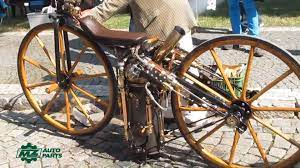
\includegraphics[scale=0.8]{Mota a vapor.jpeg}  % leia abaixo
\caption{Mota a vapor}
\label{figura:Mota a vapor}
\end{figure}

\subsection*{A introdução dos motores de combustão interna}
\vspace{1cm}
Para muitos, a invenção da moto só aconteceu a partir do momento em que os veículos de duas rodas começaram a circular com motores de combustão interna. Nesse sentido, o primeiro a fazê-lo com sucesso foi o alemão Gottlieb Daimler que, em conjunto com Wilhelm Maybach, em 1885, instalou um motor a gasolina numa bicicleta de madeira adaptada. A moto de Daimler apresentava estas características principais:
\begin{itemize}
\item Um motor a gasolina de quatro tempos do ciclo Otto com um único cilindro que se encontrava montado no centro do veículo;
\item Uma roda traseira e dianteira de igual dimensão com aros de madeira e ferro;
\item Uma roda lateral de mola em cada lado do veículo para atribuir uma maior estabilidade;
\item Um chassis com uma armação em madeira;
\item Um design pesado, áspero e desconfortável, daí ser apelidada de “quebra-ossos”;
\end{itemize}
\vspace{5cm}
O motor de combustão interna possibilitou a produção de motos à escala industrial, mas dividia a preferência dos utilizadores com os motores de dois tempos, que eram menores, mais leves e baratos. Contudo, uma das maiores dificuldades dos fabricantes de motos foi onde instalar o motor, se no selim, dentro ou sob o quadro da bicicleta ou no cubo da roda dianteira ou traseira. Inicialmente, como não havia consenso, todas as alternativas foram adotadas e só no início do século XX é que os fabricantes decidiram que o melhor local para colocá-lo seria na parte interna do triângulo formado pelo quadro. Essa foi a opção mais viável para andar de moto com segurança e mantém-se atual até aos dias de hoje.

\begin{figure}[h]
\center
 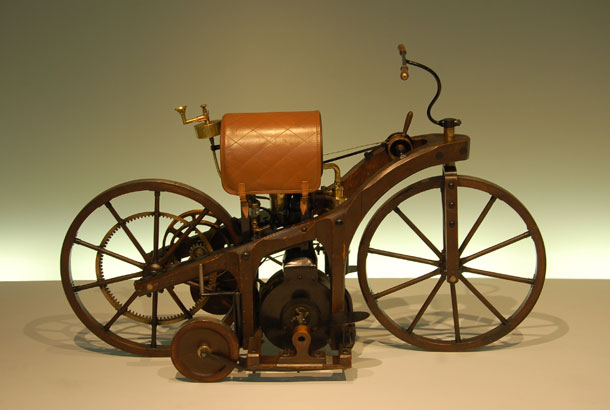
\includegraphics[scale=0.5]{Mota a combustão interna.jpeg}% leia abaixo
\caption{Mota a combustão interna }
\label{figura:Mota a combustão interna}
\end{figure}

\clearpage




\subsection{O aparecimento dos motores a 4 tempos}
Em 1895 surgiu o motor que viria a revolucionar a indústria motociclística à escala mundial, o DeDion-Bouton. Tratava-se de um motor de quatro tempos de alta rotação, leve e com meio cavalo de potência. É nesta altura que as motos passaram a ter potência e isso fez com que todos os fabricantes adotassem este novo sistema na construção dos seus modelos. Um dos exemplos mais conhecidos é o do fabricante americano Harley Davidson que passou a incorporar o motor DeDion-Bouton em todos os seus modelos.

A primeira fábrica de motos surgiu em 1894 na Alemanha e chamava-se Hildebrand e Wolfmüller. No ano de abertura foram produzidos mais de 200 veículos, o que foi um autêntico sucesso comercial. A Hildebrand e Wolfmüller também se destacou por ter sido a responsável pela criação do sistema de arrefecimento que tinha como objetivo principal o arrefecimento do motor das suas motos.

\begin{figure}[h]
\center
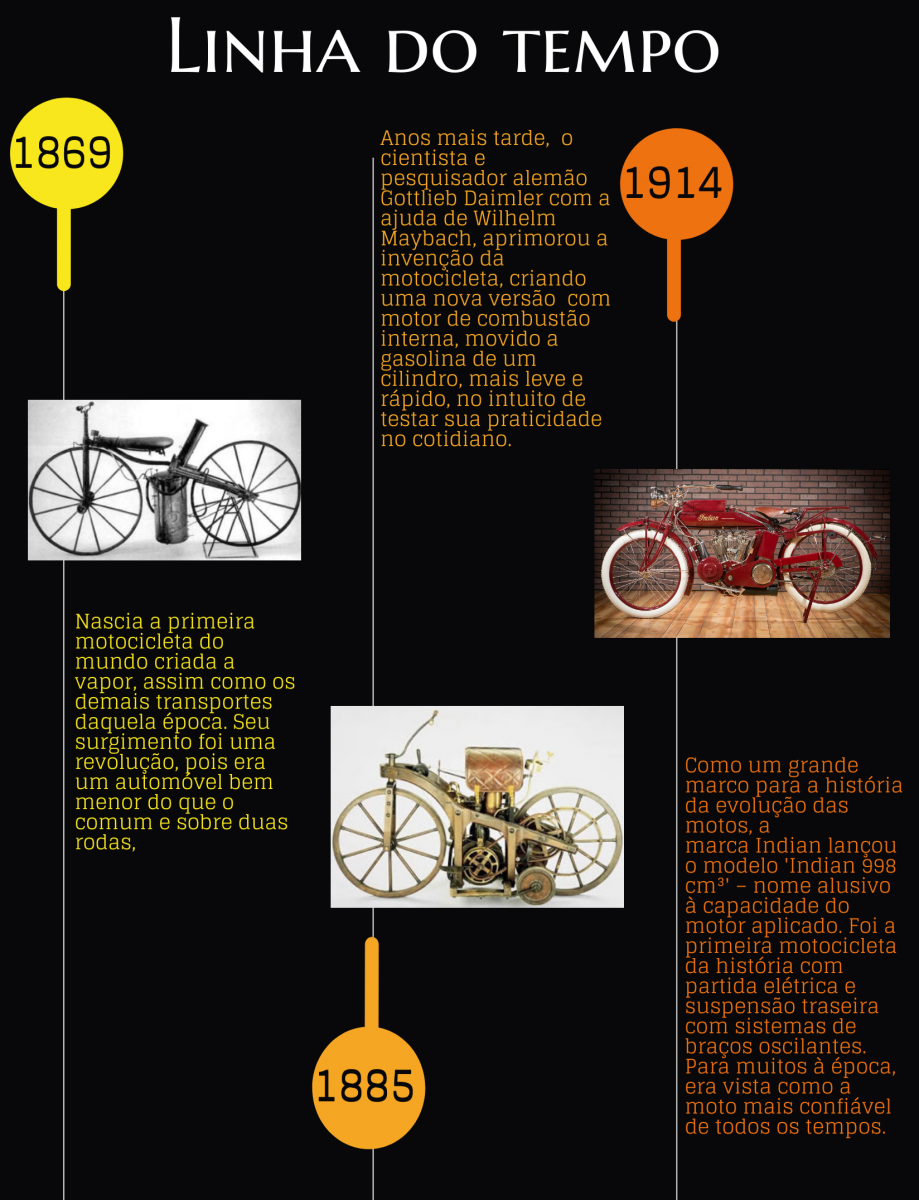
\includegraphics[scale=0.5]{linha do tempo1.jpeg} 
\caption{Linha do tempo }
\label{figura:linha do tempo}
\end{figure}

\subsubsection{A partir do século xx:}
No início do século XX assiste-se a um enorme crescimento em todo o mundo no que à produção de motos diz respeito. Na Europa existiam cerca de 43 fábricas de motos, ao passo que nos EUA, as primeiras fábricas – Columbia, Orient e Minneapolis – surgiram em 1900, chegando a 20 empresas em 1910. Este foi um período de desenvolvimento onde se introduziram todo o tipo de inovações e aperfeiçoamentos. De todas as alterações que foram realizadas a partir do século XX, evidenciam-se as seguintes:
\begin{itemize}
\item A evolução dos motores: de um a cinco cilindros e de dois a quatro tempos;
\item As suspensões foram aperfeiçoadas para oferecer um maior conforto e segurança. O destaque vai por completo para a fábrica alemã NSU que, em 1914, já oferecia a suspensão traseira do tipo mono choque como hoje é utilizada;
\item Introduziram-se os braços oscilantes na suspensão traseira das motos;
\item Os pneus passaram a ser mais resistentes; 
\item Começaram-se a utilizar os travões de disco nas provas de velocidade.
\end{itemize}
Cada fabricante procurava ser o mais original possível e isso fez com que a produção de motos evoluísse para um patamar de excelência.
\begin{figure}[h]
\center
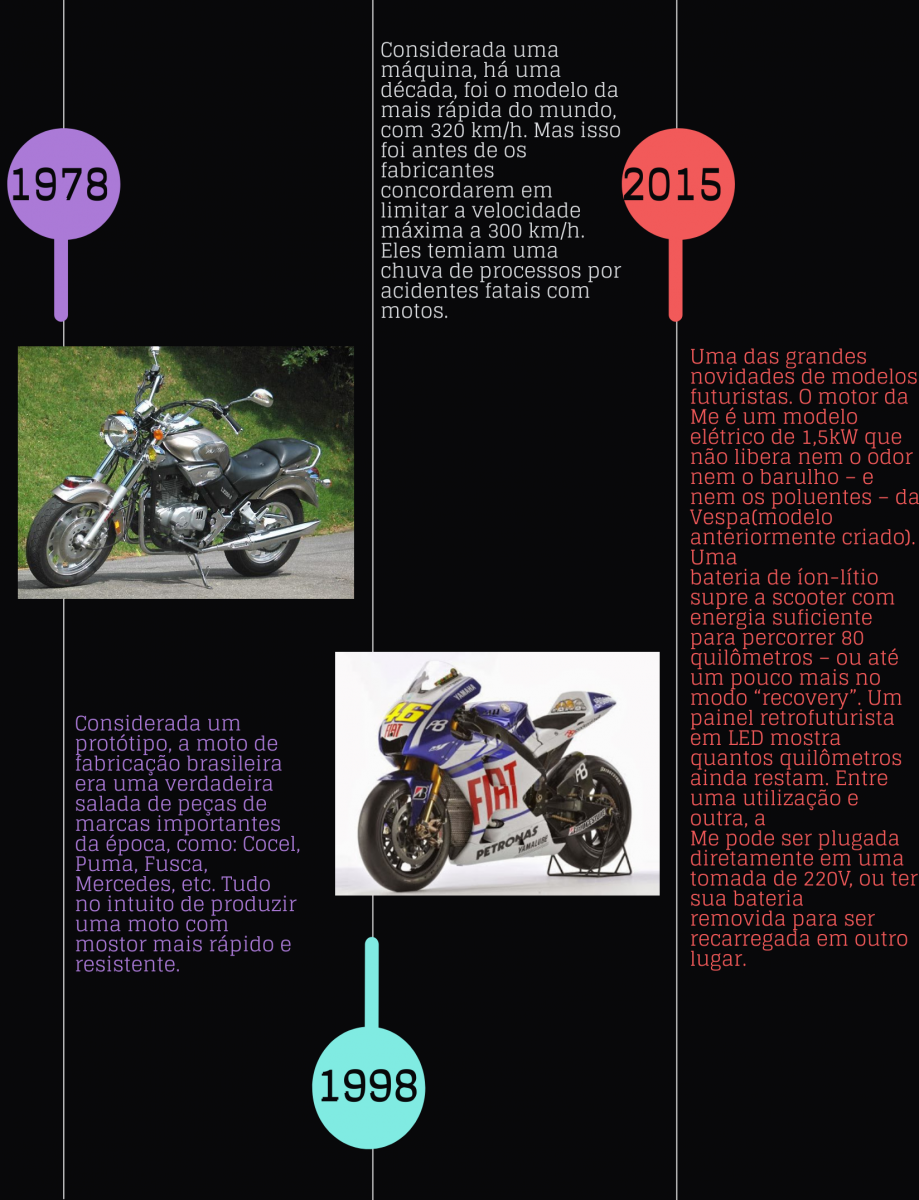
\includegraphics[scale=0.5]{linha do tempo2.jpeg} 
\caption{Linha do tempo }
\label{figura:Linha do tempo}
\end{figure}

\clearpage
\subsection{Constituintes de uma mota na atualidade}
Pretende-se, neste subcapítulo, identificar os principais sistemas/componentes dos motociclos.
\subsubsection{Quadro, forquilha e coluna de direção}
As partes fundamentais que constituem um motociclo  são o quadro, a suspensão dianteira (forquilha) e a coluna  de direção.

Quadro: O quadro ou "chassis" é constituído por uma estrutura rígida, normalmente tubular, que pode ser simples, de berço, de duplo  berço ou treliça. Ao quadro estão agregados os restantes constituintes  do veículo, tais como  motor, direção, suspensão dianteira, traseira, assento, depósito de combustível  e descanso  central e/ou lateral.

Forquilha : A suspensão dianteira ou forquilha  é o órgão que tem por  função absorver os choques causados pelas irregularidades do pavimento.  Esta suspensão pode ser de forquilha  telescópica-convencional ou invertida ou monobraço.

Coluna de direção: A coluna  de direção  estabelece a ligação  entre a suspensão dianteira  e o quadro, tendo por função articular a roda da frente (diretriz)  por acção do volante.

Alguns motociclos  já estão  equipados com um  sistema de amortecedor de direção  que permite  suavizar  a condução, quer em velocidades elevadas, quer em  velocidades baixas.
\subsubsection{Painel de instrumentos e orgãos de comando}
No painel de instrumentos situam-se os principais indicadores/instrumentos  que informam o condutor sobre o estado e condições de circulação do veículo.
Aqui listamos os principais elementos do painel de instrumentos:
\begin{enumerate}
\item Velocímetro;
\item Conta-quilómetros total;
\item Conta-quilómetros parcial;
\item Conta rotações;
\item Indicador de temperatura/Termómetro;
\item Indicador de pressão de óleo/Manómetro;
\item Amperímetro;
\item Indicador de nível de combustível;
\item Indicador de mudança engrenada;
\item Alarme de funcionamento das luzes indicadoras de mudança de direção;
\item Alarme de accionamento de luz de estrada;
\item Indicador de descanso;
\end{enumerate}
Agora listamos os principais orgãos de comando dos motociclos:
\begin{enumerate}
\item Volante;
\item Acelerador;
\item Alavanca ou manete de embraiagem;
\item Alavanca ou manete do travão dianteiro [travão de mão];
\item Alavanca do ar de arranque;
\item Interruptor de paragem  de emergência;
\item Pedal do travão traseiro [travão de pé];
\item Pedal de mudanças/selector de velocidades;
\end{enumerate}


\subsection{Motor e Sistemas}
\subsubsection{Motor}
O motor é o elemento responsável pela transformação da energia química, contida no combustível, em energia mecânica que fará o veículo deslocar-se.

Os motores normalmente utilizados nos motociclos são de explosão, podendo ser a dois ou a quatro tempos.
Vejamos as caraterísticas de cada um destes dois tipos de motores:
\begin{itemize}
\item Motores a dois tempos: Caracterizam-se por ter um ciclo de funcionamento a dois tempos. A uma rotação do motor correspondem dois tempos: 1º tempo - admissão e compressão; 2º tempo - explosão e escape;
\item Motores a quatro tempos: Caracterizam-se por ter um ciclo de funcionamento a quatro tempos distintos: 1º tempo - admissão; 2º tempo - compressão; 3º tempo - explosão ; 4º tempo - escape.
\end{itemize}
\subsubsection{Sistema de Transmissão}
Este sistema é responsável pela transmissão do movimento gerado pelo motor à roda motriz (traseira) e é constituído pela embraiagem, caixa de velocidades e transmissão.
Vejamos as caraterísticas de cada uma das componentes:
\begin{itemize}
\item Embraiagem: A embraiagem é o elemento responsável pela interrupção ou acionamento da transmissão (primária) do movimento do motor à caixa de velocidades;
\item Caixa de velocidades: A caixa de velocidades tem como função transformar o movimento que vem do motor através de várias relações (mudanças), ou interromper a transmissão do mesmo quando está em ponto morto; 
\item Transmissão: tem como função transmitir o movimento da caixa de velocidades à roda motriz (roda traseira). Tal transmissão pode ser efetuada através de corrente, correia dentada ou veio de transmissão.
\end{itemize} 
\subsubsection{Sistema de lubrificação}
Todas as peças que se movimentam e se friccionam estão sujeitas a desgaste. Por vezes há sobreaquecimento do motor, quando a velocidade de fricção é elevada, devido ao atrito provocado entre as partes. É necessário que haja lubrificação para que o atrito seja mais reduzido.
Para motores a quatro tempos é utilizado um óleo lubrificante que está depositado no cárter (parte inferior do motor) e que por ação de uma bomba é enviado sob pressão para os diversos pontos do motor. Este motor é designado como motor de cárter húmido.
Por sua vez, nos veículos com motores a dois tempos, o óleo lubrificante é misturado com a gasolina no acto de abastecimento do veículo. Neste caso o motor é designado como motor de cárter seco.
\subsubsection{Sistema de referigeração}
Para manter uma temperatura ideal no motor é necessário dissipar, através das alhetas, parte do calor que se gera por o motor estar em funcionamento. Isso é feito através de um sistema de refrigeração, que pode ser por ar direto, ar forçado ou líquido de refrigeração.
No caso de refrigeração por ar direto, a zona exterior do(s) cilindro(s) e das câmaras de explosão possui alhetas ou nervuras para aumentar a superfície de irradiação de calor, sendo arrefecidas por circulação de ar durante a deslocação do veículo.
Em alguns motociclos, o motor possui uma blindagem exterior que envolve as alhetas, fazendo-se o seu arrefecimento por circulação de ar forçado, com o auxílio de uma turbina.
No arrefecimento por líquido de refrigeração (habitualmente água), o motor está equipado com um circuito onde o mesmo, através de uma bomba, garante o arrefecimento. Quando o líquido de refrigeração atinge determinada temperatura existe uma válvula (termóstato) que permite a sua passagem, através de tubagens, para o radiador. Com o auxílio de uma ventoinha eléctrica, esse líquido vai ser arrefecido para voltar, na temperatura ideal, ao circuito de arrefecimento.
\subsubsection{Sistema de Alimentação}
O sistema de alimentação tem como função fazer descer a gasolina, contida no depósito de combustível, através de tubagem, até ao carburador. A alimentação é feita por efeito da gravidade, uma vez que o depósito se encontra colocado a um nível superior ao carburador/motor.
Na ligação do depósito de combustível ao carburador existe uma torneira que pode ser de comando manual ou automático. No primeiro caso, quando é atingido o nível de reserva, o condutor altera a posição de entrada (aberto) para a posição de reserva. O carburador é o elemento responsável pela mistura da gasolina com o ar na proporção adequada. Em alguns sistemas de alimentação atuais, o carburador é substituído pela bomba de injeção.
Através da válvula de admissão, a mistura gasolina/ar passa para o cilindro, onde se dá a explosão, produzindo-se a energia mecânica que fará o veículo deslocar-se.
\subsubsection{Sistema de Direção}
O sistema de direção tem como função orientar a roda da frente (diretriz) por ação do guiador, de modo a que o condutor consiga direcionar o mesmo no sentido pretendido, cuja direção é direta e, por isso, proporcional à forma brusca ou suave com que o manobramos. De modo a desencadiar uma condução mais suave, já existem motociclos equipados com um sistema de amortecedor de direção.
Quanto maior for o avanço da coluna de direção, maior será a estabilidade do veículo, favorecendo a sua utilização em estrada. Em contrapartida, um menor avanço da coluna de direção, favorecerá o seu manosiamento, de forma a adequar a sua utilização aos meios urbanos.
\subsubsection{Sistema Elétrico}
O sistema elétrico tem por base uma bateria que funciona como acumulador de energia elétrica, produzida pelo gerador (alternador ou dínamo), que é fornecida a todos os órgãos elétricos do veículo.
Existem baterias com manutenção e baterias sem manutenção. Nas baterias com manutenção deve-se, com regularidade,verificar o nível de  eletrólito (água destilada + ácido sulfúrico) já que a água destilada tende a evaporar-se. Se for necessário, deve adicionar-se apenas água destilada pelos orifícios existentes na parte superior da bateria. As baterias sem manutenção quando chegam ao fim do seu ciclo de vida devem ser entregues em locais próprios para o efeito, a fim de proteger o meio ambiente.
\subsubsection{Sistema de Travagem}
Este sistema é composto por dois travões de serviço. Um travão de mão que actua sobre a roda da frente (normalmente de disco) e outro travão de pé que actua sobre a roda da retaguarda(pode ser de disco ou de tambor).
Geralmente, os travões dos motociclos são hidráulicos(acionados através de fluído designado por óleo dos travões).
Os travões de disco, crescentemente utilizados, possuem uma maior eficácia na travagem em relação aos travões de tambor, pois,por terem uma utilização exclusivamente exterior permitem um maior e mais rápido arrefecimento do sistema, bem como uma maior força de travagem.
\subsubsection{Sistema de Suspensão}
O sistema de suspensão filtra as irregularidades do pavimento, para proteger o veículo de possíveis vibrações, solavancos ou ressaltos e proporciona um maior conforto ao condutor e eventual passageiro, uma vez que mantém em simultâneo as rodas em contacto permanente com o solo.
O sistema de suspensão(dianteiro e traseiro) é composto por pneus, molas e amortecedores.
\subsubsection{Sistema de Arranque}
Ao sistema de arranque cabe a responsabilidade de colocar em funcionamento o motor.Existem dois tipos de sistemas de arranque: sistema de arranque por pedal (com ou sem descompressor) e sistema de arranque elétrico.
O sistema de arranque por pedal, ao ser impulsionado com o pé transmite movimento ao motor para iniciar o seu funcionamento. Devido à taxa de compressão e/ou elevada cilindrada, alguns motociclos possuem um descompressor, facilitando o arranque.
O sistema de arranque elétrico tem por base um motor elétrico. Este ao ser acionado através de um interruptor situado junto do punho direito do guiador, aciona o funcionamento do motor.
\subsection{Nova geração motas elétricas}
Devido ao significativo aumento da necessidade de estar em diferentes sítios, o mais rapidamente possível, ao longo do dia de cada pessoa, quer seja para o trabalho, ir às compras entre várias outras coisas, o aumento da poluição, quer sonora, quer do ar, cresceu exponencialmente.
A poluição causada pela emissão de CO2 proveniente dos motores alimentados por combustíveis fosseis é uma das maiores causas do aparecimento de doenças e do aumento do efeito de estufa. Para melhorar este aspeto, a invenção das motas elétricas foi um grande marco na atualidade e na evolução da respetiva indústria. Mas afinal como é que funcionam as motas elétricas? A base de construção de uma mota é: a bateria, a ignição, motor elétrico e os acessórios. A bateria é a fonte de alimentação da mota e é constituída por um gerador de tensão capaz de manter a bateria sempre carregada; os fios estão encarregues de levar a energia a cada parte da mota e o regulador de tensão que serve para evitar sobrecargas. Por fim o motor elétrico converte energia elétrica em movimento físico, gerando campos magnéticos onde circula uma corrente, de seguida, o campo magnético causa uma força com um íman que aciona o motor.   
Apesar das grandes vantagens, o custo de uma mota elétrica ainda é bastante elevado sendo assim pouco acessível a qualquer pessoa, ainda assim, prevê-se um crescimento global de 35 \% na área das motas elétricas, sendo a Europa a região com mais vendas. Este crescimento deve-se principalmente á evolução tecnológica, ao aumento da popularidade dos veículos elétricos e os incentivos governamentais.



\subsection{Novas descobertas no ramo das motas elétricas}
A maioria das motas elétricas contém o motor instalado na parte central, mas uma nova abordagem promete alterar isso, este novo modelo denomina-se por modelo de Hubless e tem como objetivo subjacente instalar o motor no aro traseiro. Esta solução visa eliminar toda a estrutura da roda, reduzindo a massa suspensa da mota, além disso, proporciona eficiência na transferência de torque e potência. 
Até agora existem vários modelos, mas cinco deles têm-se destacado pela sua qualidade e performance, sendo eles : Mota NUUK Urban e Tracker (velocidade máxima de 105 Km/h e autonomia de 60 Km), BMW C Evolution (velocidade máxima de 129 Km/h e autonomia de 160 Km), RMK E2 (velocidade máxima de 160 Km e autonomia de 300 km), Vespa Elettrica (velocidade máxima de 30 Km e autonomia de 100 Km) e por fim a mota elétrica Curtiss Motorcycles Zeus (velocidade máxima 220 Km/h e autonomia de 450 Km) este modelo está pronto para ser produzido mas ainda não foi colocado á venda. Os preços destes modelos podem circular entre os 7.000 euros e os 53.000 euros.

\begin{figure}[h]
\center
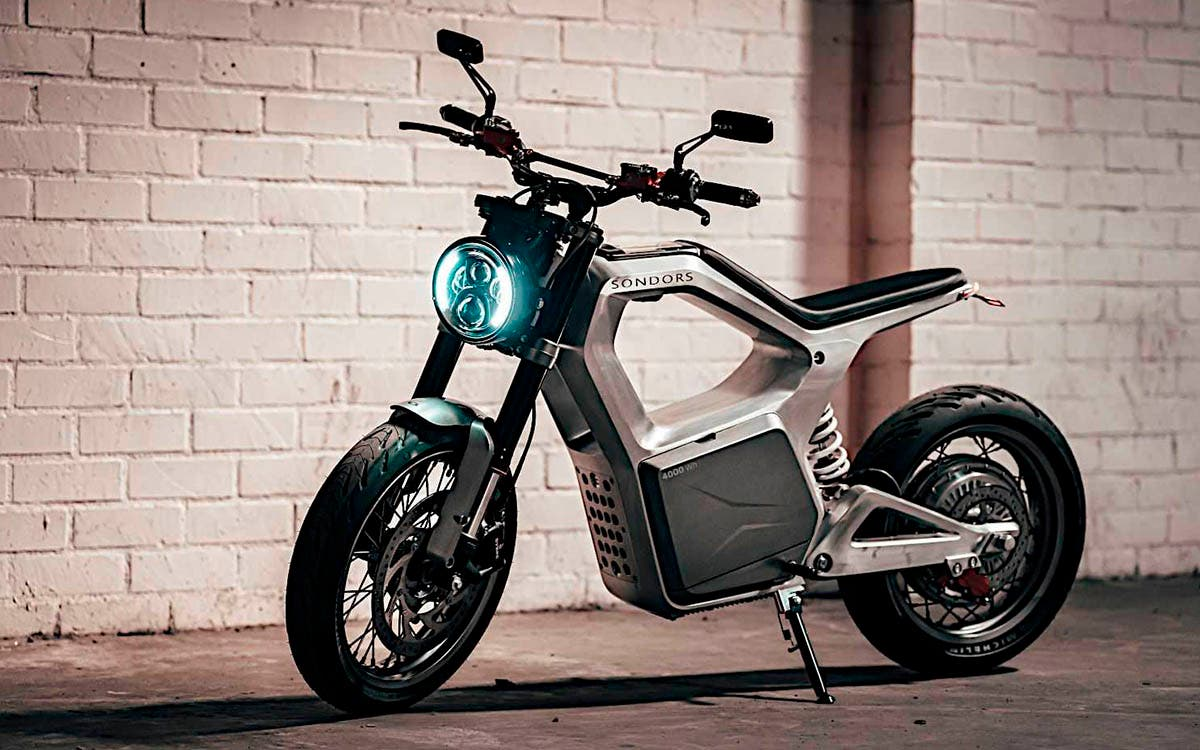
\includegraphics[width=5cm]{motaeletrica.jpeg} % leia abaixo
\caption{Mota elétrica}
\label{figura:motaeletrica}
\end{figure}


\subsection{Moto GP}
A partir do século XX começaram-se a disputar Grandes Prémios de Motociclismo em vários países, mas com o início da Segunda Guerra Mundial só algum tempo após o fim é que surgiu combustível disponível para criar uma verdadeira competição internacional.
Foi assim, em 1949, que ocorreu a primeira competição dividida em quatro categorias a solo: 500cc, 350cc, 250cc, 125c. Em 1949, o vencedor foi Leslie Graham pela equipa AJS Company, usando o modelo AJS Porcupine que inicialmente foi construída para ser superalimentada, mas em 1946 o FCIM proibiu a superalimentação. O motor E90S Porcupine era uma construção unitária,500cc, duplo DOHC, com cilindros e cabeçotes horizontais, para dar à mota um centro de gravidade baixo. Uma versão posterior deste motor foi chamada de E95, projetada para ter os cilindros inclinados a 45 graus para melhorar o resfriamento e facilitar a instalação do carburador. A saída da caixa de câmbio de quatro velocidades estava à direita. Conforme projetado originalmente, o E90S deveria ser superalimentado, com o soprador montado acima da caixa de marchas e acionado pela embraiagem. A principal mudança inicial foi reduzir o ângulo da válvula para 90 graus para uma câmara de combustão mais compacta. Tinha dois carburadores GP montados em borracha, inclinados a 49 graus, com um sistema de tanque flutuante incomum usado em vez de bacias flutuantes. Mais tarde o motor foi então acionado para que funcionasse sem um supercharger e Leslie correu com ela obtendo a primeira e única vitoria da equipa AJS no campeonato do mundo.  A partir daí os vencedores pertenceram sempre a equipas italianas visto que estas dominaram os campeonatos do mundo no século 50. A MV Agusta, da equipa Scuderia MV Agusta, era uma mota de 4 cilindros e 750cc que venceu o campeonato do mundo 17 vezes seguidas, provando a sua dominância na época. Em 2002 surgiu finalmente a famosa Moto GP que consiste em 18 provas em 14 países diferentes e veio substituir a categoria 500cc e que atualmente é de 1000cc devido á evolução constante da indústria de competição, sendo atualmente a marca Yamaha a construtora campeã, mas, apesar de ser a atual equipa campeã, a Honda tem mais títulos, 16. Para podermos comparar alguns valores, a velocidade máxima a ser atingida numa corrida antigamente era de 120 km/h e atualmente já atingiu os 362 km/h. As motas utilizadas em Moto GP nos dias de hoje são maioritariamente produzidas por marcas japonesas como a Yamaha, Honda e Suzuki. 

\begin{figure}[h]
\center
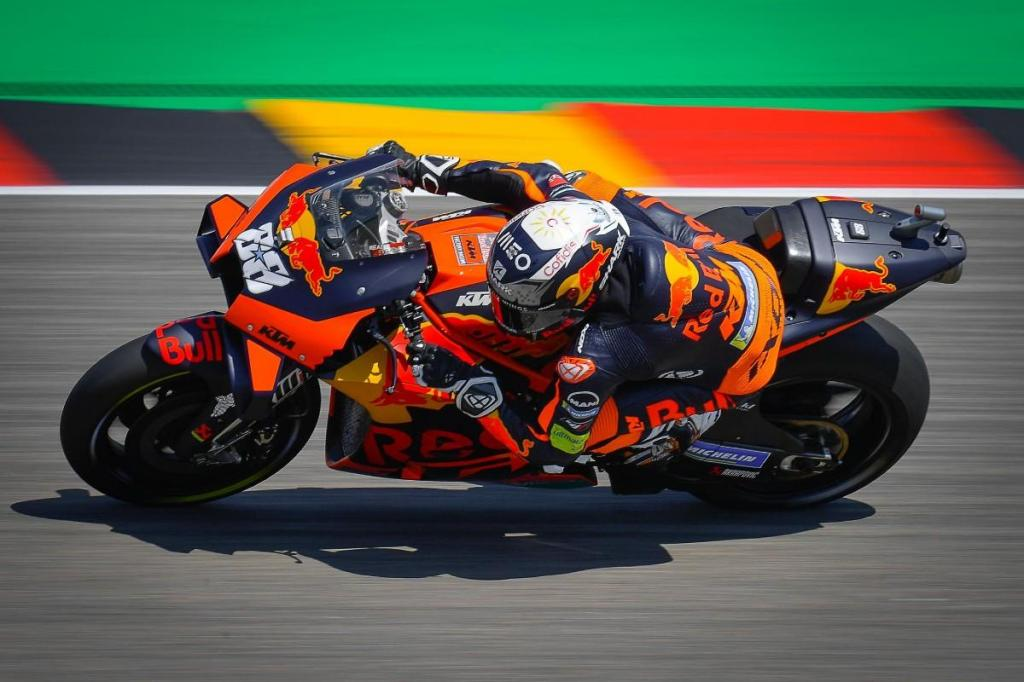
\includegraphics[width=5cm]{motogp.jpg} % leia abaixo
\caption{Moto GP}
\label{figura:motogp}
\end{figure}


%Fazer tabela com os últimos vencedores ano/vencedor
\begin{table}[h]
\center

\begin{tabular}{r|r |lr}

Ano & Vencedor & Equipa\\ % Note a separação de col. e a quebra de linhas
\hline                               % para uma linha horizontal
 2021   &  Fabio Quartararo  & Yamaha \\
 \hline
 2020 &  Joan Mir & Suzuki \\
 \hline
 2019 & Marc Márquez & Honda \\
 \hline 
 2018 & Marc Márquez & Honda \\
 \hline 
 2017 & Marc Márquez & Honda \\ 
 \hline
 2016 & Marc Márquez & Honda \\
 \hline 
 2015 & Jorge Lorenzo & Yamaha\\
 \hline
 2014 & Marc Márquez & Honda \\
 \hline
 2013 & Marc Márquez & Honda \\
 \hline
 2012 & Jorge Lorenzo & Yamaha\\
 \hline
 2011 & Casey Stoner & Honda \\
 \hline
 2010 & Jorge Lorenzo & Yamaha\\
 
 
\end{tabular}
\caption{Vencedores do Moto GP nos últimos anos}
\label{tabela}
\end{table}

\subsection{Riscos e vantagens do motociclo enquanto meio de transporte}
A caraterização da moto como um transporte inseguro e que envolve maior risco remete, sobretudo, para aspetos relacionados com o seu \textit{design}. A ausência de proteção física é, de certa forma, a maior preocupação associada à probabilidade de sofrer um acidente, sobretudo, pelas lesões que dele podem decorrer.Contudo, a mota não tem vida própria e não podemos partir do pressuposto de que todos os acidentes ocorrem devido a fatores externos ao condutor. Desta forma, a representação do risco terá, também, que ser analisada à luz das condutas de utilização por parte dos motociclistas e, até mesmo, das condições em que se encontram as vias de circulação, o trânsito existente e as situações de imprudência em que o motorista, por vezes, coloca o veículo.
\begin{figure}[h]
\center
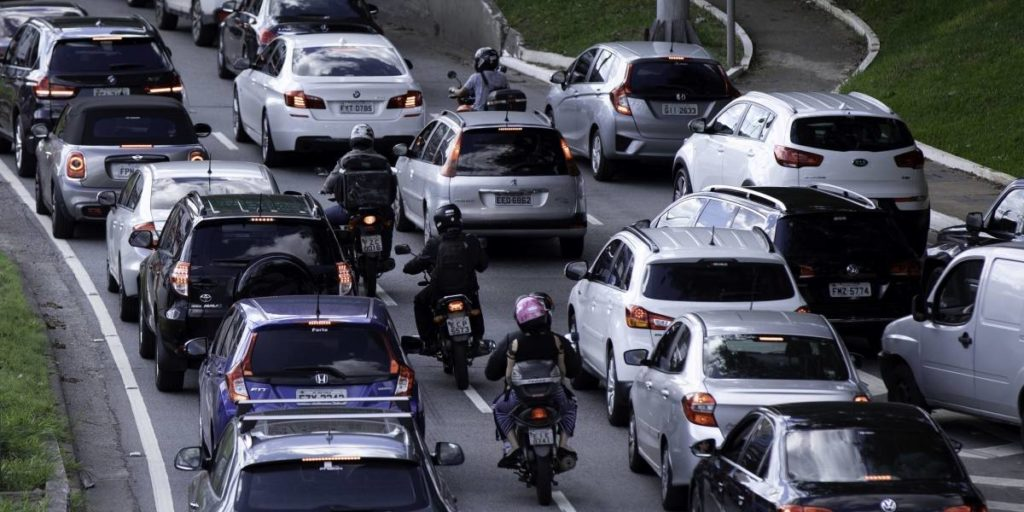
\includegraphics[width=5cm]{condução perigosa.jpg} % leia abaixo
\caption{Condução Perigosa}
\label{figura:Condução Perigosa}
\end{figure}
Para além disso, muitos estudos apontam que uma grande percentagem de acidentes com motos está associada a motociclistas, que utilizam este veículo como instrumento de trabalho. De facto, pela sua agilidade motora, reduzido consumo de combustível e maior facilidade de estacionamento em meio urbano, muitos são os profissionais que utilizam a moto no exercício da sua profissão. Contudo, para muitos destes profissionais, que vão desde a área da restauração, forças de segurança…, a jornada de trabalho pode ser extensa, o que, também, os deixa mais expostos aos perigos.

O ser mais prático associado ao ser mais barato, pode, caso não exista uma atitude de ponderação de risco prévia, conduzir a uma incursão em situações de perigosidade associadas ao uso das motas.
\begin{table}[h]
\center

\begin{tabular}{r|r |lr}

Ano & Número de acidentes de motociclos:\\ % Note a separação de col. e a quebra de linhas
\hline                               % para uma linha horizontal
 2021 & 38823 \\
 \hline
 2020 & 36237 \\
 \hline
 2019 & 33157 \\
 \hline 
 2018 & 28861 \\
 \hline 
 2017 & 22115 \\
 \hline
 2016 & 16035 \\

 
\end{tabular}
\caption{Número de acidentes de motociclos nos últimos anos}
\label{tabela}
\end{table}

Na extremidade oposta às situações supranumeradas, surge-nos, por exemplo, a sensação única de sentir o vento nos cabelos e uma comunhão perfeita com a natureza, que levam muitos aficionados a adquirir e promover o uso da mota, enquanto veículo de lazer, por excelência.

Aqui as vantagens enumeradas passam por se trata de veículos que, sobretudo em viagens mais longas, consomem consideravelmente menos combustível do que um carro, implicam menos reparações e mais baratas. Ao contrário do automóvel, as trocas de óleo são relativamente simples e podem ser feitas pelo proprietário e não por um mecânico especializado. Relativamente ao estacionamento, é frequente existirem lugares específicos de estacionamento apenas para motocicletas e com menor ocupação do que os destinados aos carros, por exemplo. Acresce, ainda, referir que o registo e os impostos para as motocicletas são consideravelmente menos dispendiosos do que para os restantes veículos.

Do exposto, cumpre-nos concluir que na utilização da moto, enquanto meio de transporte, quer numa vertente laboral ou de lazer, o risco (desvantagens) não de dissocia das vantagens. No entanto, a linha ténue, mas que faz toda a diferença no manuseio apelida-se de uso seguro e responsável.

\begin{figure}[h]
\center
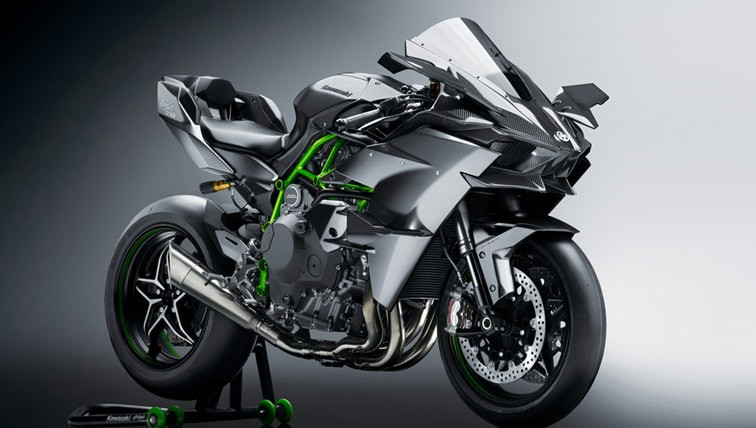
\includegraphics [scale=0.5]{mota mais potente do mundo.jpg} % leia abaixo
\caption{A Verdadeira Mota}
\label{figura:"A Verdadeira Mota"}
\end{figure}


\chapter{Conclusão}
Com o presente trabalho pretendeu-se, através da aplicação metodológica com recurso ao LATEX, dar a conhecer a evolução significativa que um meio de transporte como o motociclo conheceu, ao longo da sua existência.Estamos perante um grande desenvolvimento que representa, na atualidade, um reconhecido poder.A sua notória necessidade no quotidiano das pessoas, que se deslocam cada vez mais rápido e com uma elevada frequência, torna o seu uso recorrente. Por outro lado, o facto do aumento do seu uso provocar um consequente aumento dos níveis de poluição, é uma contrariedade que, como vimos na presente investigação, está, nos dias de hoje, a ser combatida com a invenção e modernização das motas elétricas, que futuramente vão colocar o planeta a salvo de uma grande percentagem de gases. Com este relatório ficámos, também, a conhecer a constituição mecânica de uma mota, entendendo melhor o seu funcionamento.

Da abordagem feita à competição/desporto associados às motos, concluímos que a indústria de competição, aqui concretizada na Moto GP, é uma atividade que envolve quantias avultadas de dinheiro devido ao grande número de espectadores e à ávida vontade de cada equipa em ganhar.

Num breve capítulo para o efeito, tratámos o sentir da condução responsável e alguns cuidados a ter com o objetivo último da redução dos perigos e sinistralidade associados aos motociclos. Verificou-se, assim, que este tipo de veículos de cariz utilitário e de lazer, aos quais está associada uma elevada taxa de risco, poderá ver os mesmos reduzidos se o seu manuseio se pautar por princípios de responsabilidade, potenciando-se, desta forma, as vantagens do uso das motas.


\label{chap.conclusao}
\chapter*{Contribuições dos autores}
A elaboração deste relatório contou com a participação dos autores em absoluto espírito de cooperação.

Começaram por ser programados momentos de atividade investigacional sobre a temática a tratar. Aos quais se seguiu a definição do título e da estrutura funcional do relatório.

Após a recolha de toda a informação, iniciou-se a execução, que obedeceu aos pressupostos de um trabalho de equipa: apresentação de pontos de vista, discussão,respeito pelas pontuais divergências de opinião entre cada um dos autores e registo da informação. Além do registo escrito, que suporta o relatório, os autores cooperaram na introdução de tabelas, imagens, diferentes listas de numeração, entre outros conteúdos pertinentes.

Foi, ainda, feito um trabalho de campo de cariz mais prático investigacional, que contemplou o contacto direto com familiares de um dos autores deste relatório. Trata-se de alguém que detém uma grande experiência na condução e posse de motociclos.

Sendo, aqui, de realçar que o próprio autor visado, também, teve oportunidade de, no contexto de execução do trabalho, partilhar a sua própria experiência, enquanto motociclista e utilizador frequente deste meio de transporte.

Deste modo, através do recurso à experiência pessoal e a diversas fontes de informação, das quais destacamos artigos científicos,publicações em jornais e sites, foi possível desenvolver conhecimentos, que aplicámos na execução do relatório em LATEX. Aqui, foi fundamental o contributo do docente António Manuel Adrego da Rocha para a aquisição de competências, que nos possibilitaram aplicar esta opção metodológica no presente relatório e esclarecer dúvidas que, na sua implementação, foram surgindo.
\chapter{Acrónimos}
\begin{acronym}
\acro{ua}[UA]{Universidade de Aveiro}
\acro{leci}[LECI]{Licenciatura em Engenharia de Computadores e Informática}
\acro{glisc}[GLISC]{Grey Literature International Steering Committee}
\end{acronym}

\begin{thebibliography}{6}
\bibitem{Moto GP}

\textit{https://pt.wikipedia.org/wiki/MotoGP}

Moto GP

\bibitem{latex}

\textit{https://pplware.sapo.pt/tutoriais/o-que-e-o-latex/}

Latex

\bibitem{Evolução das motas}

\textit{//sites.google.com/site/desporto2rodas/historia-e-evolucao-das-motas}

Evolução das motas

\bibitem{3}

\textit{https://pt.wikipedia.org/wiki/MV-Agusta}

MV Agusta

\bibitem{4}

\textit{https://www.motosport.com.pt/moto-gp/motogp/motogp-historia-leslie-graham-o-primeiro/}

Moto GP


\bibitem{5}

\textit{https://www.zev.news/article/125/estudo-indica-crescimento-global-de-35-das-motos-eletricas-ate-2024}

Motas elétricas

\bibitem{6}

\textit{https://www.scielo.br/j/icse/a/yK6JyjsVxxNnHtwWLfDhR4D/abstract/?lang=pt}

Segurança nos Motociclos
\end{thebibliography}



\end{document}
